The time-frequency spectrogram is a form of representation of the micro-Doppler signatures. It presents the characteristics of human activity in the time-frequency domain. Feature extraction in micro-Doppler analysis is used to reduce the number of features of a spectrogram; the aim is to identify features of the signal, which are required for recognizing an activity, and to disregard other parts as background noise. A good feature extraction technique is a very important component in a recognition system; because those extracted features will be fed into the classification algorithms and this will dictate the quality of the classification and the time that the classifiers will take to sufficiently train the model. For classifying different activities, it is required to extract features from the spectrograms and use these features to train the machine learning algorithms, such as SVM, and \textit{k}NN to differentiate the activities.

Two-directional Two-dimensional Principal Component Analysis was firstly developed by \cite{zhang20052d} and used for face representation and recognition. The authors of \cite{tivive2013image} applied 2D2PCA for micro-Doppler features extraction and compared it with Gabor Wavelet Filter, Mel-frequency Cepstral Coefficients, Cadence Frequency based method, and Empirical Mode Decomposition. The performance of 2D2PCA exceeded all the others significantly, which is the reason why it is used in this research.

PCA is well-known as a classic feature extraction and dimensionality reduction technique \cite{wold1987principal}. A spectrogram is an image composed of a two-dimensional structure of pixels. In order to use PCA, firstly the two-dimensional image of the spectrogram must be transformed into a one-dimensional vector. 2D2PCA can be regarded as a two-dimensional version of the PCA, 2D2PCA performs feature extraction on the rows and columns of an image simultaneously and it is more efficient in computing the covariance matrices, the eigenvalues and the eigenvectors than PCA alone.

A spectrogram generated by STFT can be denoted by a matrix $A\in R^{m \times n}$, where $R$ indicates  that the elements of A consist entirely of real numbers. Let  $X\in R^{n\times d},n \geq d$ be a projection matrix with orthonormal components. $Y\in R^{m\times d}$ is generated by projecting $A$ onto $X$, which can be written as $Y=AX$. The reduction of the dimensionality is achieved by the selection of a suitable value for $d$, which decides how many features will be kept in each row, also is the final number of columns after the projection.   

Matrix $Y$ must preserve relevant information of the specific activity contained in the spectrogram. An ideal projection matrix should ensure that the result after the projection is very distinct from others of different activities. This makes the samples of different activities more independent to each other so that they do not cluster together. Therefore, it is beneficial to the classification if the most relevant information is kept after projection. In order to determine a good projection matrix $X$, the following criterion \cite{zhang20052d} is adopted:
\begin{equation}
\label{eq:llk}
\begin{split}
&J(X)=trace\{E[(Y-EY) (Y-EY)^T ]\} \\&=trace\{E[(AX-E(AX))(AX-E(AX))^T ]\}\\&=trace\{X^T E[(A-EA)^T (A-EA)]X\},
\end{split}
\end{equation}
where $J(\cdot)$ is an objective function. In order to find the optimal projection matrix X, it is required to maximize $J$. $E$ is the expectation operator that when applied to a matrix produces a new matrix containing the expected values of the elements of the original matrix. The last term in Eq. (\ref{eq:llk}) follows the commutative property of matrices where $trace(QP)=trace(PQ)$, $Q$ and $P$ represent any two matrices. 

The covariance matrix \cite{zhang20052d} of $A$ is defined as:
\begin{equation}
G=E[(A-EA)^T (A-EA)], 
\end{equation}
Suppose that the training set consists of $M$ spectrograms $\{A_1,A_k,\ldots,A_M\}$, the covariance matrix  $G$ can be computed as:
\begin{equation}
G=(1/M) \sum_{k=1}^{M}〖(A_k-\bar{A})^T (A_k-\bar{A})〗,
\end{equation}
where $\bar{A}$ is the average spectrograms as $\bar{A}=(1/M) \sum_{k=1}^{M}A_k$.
Eq. (\ref{eq:llk}) can be simplified as:
\begin{equation}
J(X)=X^T GX,
\end{equation}
Let $A_k=〖[(A_k^{(1)} )^T (A_k^{(2)} )^T\ldots〖(A_k^{(m)})〗^T]〗^T$ and $\bar{A} ̅=〖[(\bar{A}^{(1)} )^T (\bar{A}^{(2)} )^T\ldots〖(\bar{A}^{(m)})〗^T]〗^T$, where $A_k^{(i)}$ and $\bar{A}^{(i)}$ denote the $i_{th}$ row of $A_k$ and the $i_{th}$ row of $\bar{A}$, respectively. The covariance matrix  $G_r$ can be rewritten as:
\begin{equation}
G_r=(1/M) \sum_{k=1}^{M}\sum_{i=1}^{m}〖(A_k^{(i)}  -\bar{A}^{(i)} )^T (A_k^{(i)}  -\bar{A}^{(i)})〗,
\end{equation}

The covariance matrix $G_r$ is essentially the same as $G$, the only difference is that matrix $A$ is taken as a set of row vectors. Through diagonalization of covariance matrix $G_r$, the ideal projection matrix $X$ can be obtained.

In the same way, matrix $A$ also could be taken as a set of column vectors. Let $A_k=[(A_k^{(1)} )(A_k^{(2)})\ldots(A_k^{(n)})]$ and $\bar{A}=[(\bar{A}^{(1)})(\bar{A}^{(2)} )\ldots(\bar{A}^{(n)})]$, where $A_k^{(j) }$ and $\bar{A}^{(j)}$ denote the $j_{th}$ column of $A_k$ and the $j_{th}$ column of $\bar{A}$, respectively. The covariance matrix  $G_c$ could be rewritten as:
\begin{equation}
G_c=(1/M) \sum_{k=1}^{M}\sum_{j=1}^{n}〖(A_k^{(j)}  -\bar{A}^{(j)} ) (A_k^{(j)}  -\bar{A}^{(j)})^T〗,
\end{equation}

Let $Z\in R^{m \times q}$ be a matrix with orthonormal columns.  Projecting matrix $A$ onto $Z$ yields matrix $B=Z^T A,B\in R^{q \times n}$. The reduction of the dimensionality is achieved by the selection of a suitable value for $q$, which determines how many features will be kept in each column, it also corresponds to the number of rows of $B$. $Z$ can be obtained through diagonalization of $G_c$.

After the projection matrices $X$, $Z$ are obtained, $A$ must be projected onto $X$ and $Z$ simultaneously in order to yield a matrix $C$:
\begin{equation}
C=Z^T AX,
\end{equation}
the matrix $C$ is called the \textit{coefficient matrix}. It can be taken as the input features that are fed into SVM and $k$NN classifiers.
\begin{figure}[!t]
\centering
%\captionsetup{justification=centering}
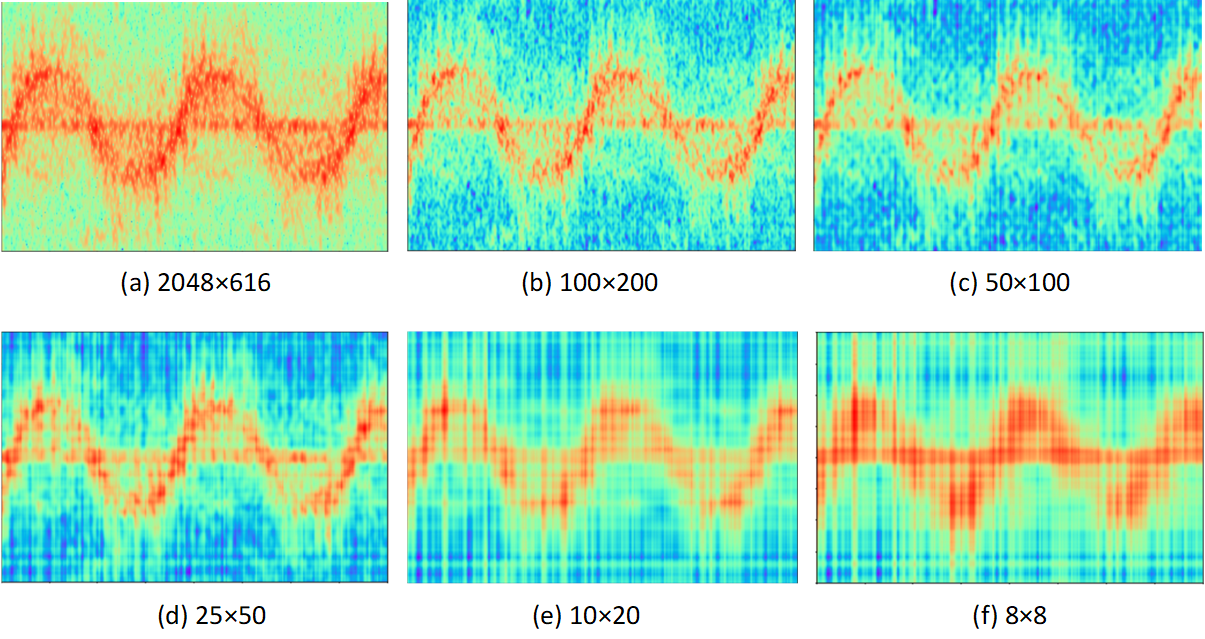
\includegraphics[width=3.6in]{pca2d2}
\caption{Dimensionality reduction with 2D2PCA}
\label{fig_tf}
\end{figure}

Fig. \ref{fig_tf}(a) is a spectrogram whose size is $2048\times 616$ pixels. It is the result of an echoed radar signal of a human walking indoors. The method 2D2PCA was applied on this original spectrogram for different row and column dimension reductions. The results are shown in Fig. \ref{fig_tf}(b) and Fig. \ref{fig_tf}(c). We note that Fig. \ref{fig_tf}(b) and Fig. \ref{fig_tf}(c) still retain detailed time-frequency characteristics (the periodic waves), but the image dimensions are well reduced, visually they are almost the same as the original spectrogram. Even when reducing the dimensionality to 8 rows and 8 columns the remained characteristics still can reflect the periodic trend of a human walking as it can be seen in Fig. \ref{fig_tf}(f). 2D2PCA is able to keep most of the distinctive features (pixels) while greatly reducing the dimensions of the micro-Doppler signatures.